\documentclass[9pt,twoside]{pnas-new}

\templatetype{pnasmathematics} 

\title{PNAS LaTeX Template for preparing single-column mathematics articles on Overleaf}

% Authors should be listed in alphabetical order by last name. Use letters to indicate affiliations.
\author[a]{Author One}
\author[a]{Author Two} 
\author[a]{Author Three}

\affil[a]{University of California, Los Angeles}

% Please give the surname of the lead author for the running footer
\leadauthor{First author last name} 

% Please add a significance statement to explain the relevance of your work
\significancestatement{Authors must submit a 120-word maximum statement about the significance of their research paper written at a level understandable to an undergraduate educated scientist outside their field of speciality. The primary goal of the significance statement is to explain the relevance of the work in broad context to a broad readership.}

% Please include author contributions here.
\authorcontributions{Please provide details of author contributions here.}

% Please provide three to five keywords, separated by the pipe symbol. Keywords will signal the application, methods, etc. to the reader.
\keywords{Keyword 1 $|$ Keyword 2 $|$ Keyword 3 $|$ ...} 

\begin{abstract}
Please provide an abstract of no more than 250 words in a single paragraph. Abstracts should explain to the general reader the major contributions of the article. References in the abstract must be cited in full within the abstract itself and cited in the text.
\end{abstract}

\dates{This manuscript was compiled on \today}
\doi{Math 168 Spring 2020 Final Project}

\begin{document}

\maketitle
\thispagestyle{firststyle}
\ifthenelse{\boolean{shortarticle}}{\ifthenelse{\boolean{singlecolumn}}{\abscontentformatted}{\abscontent}}{}

% If your first paragraph (i.e. with the \dropcap) contains a list environment (quote, quotation, theorem, definition, enumerate, itemize...), the line after the list may have some extra indentation. If this is the case, add \parshape=0 to the end of the list environment.
\dropcap{T}his PNAS journal template is provided to help you format your project correctly. Instructions for use are provided below. 

Note: please start your introduction without including the word ``Introduction'' as a section heading (except for math articles in the Physical Sciences section); this heading is implied in the first paragraphs. 

\section*{Guide to using this template on Overleaf}

Whether using this template on Overleaf or locally, make sure that you copy all of the files (.sty, .bst, .cls, etc.) so that the formatting will be maintained for your project. You should only need to edit this file (.tex), the bibliography (.bib), and add figures.

If you have a question while using this template on Overleaf, you can use the help menu (``?'') on the top bar to search for \href{https://www.overleaf.com/help}{help and tutorials}. The instructor and TA are available to help with LaTeX-related questions and Piazza discussion on these topics is encouraged.

\subsection*{Organizing your write-up}

You should use sections to divide up your project into sections. Subsections like this one can be helpful to further organize your work. 

\subsection*{Submitting Project}

A PDF of the project should be submitted via Gradescope. Only one project needs to be submitted per group.

\subsection*{Format}

Many authors find it useful to organize their manuscripts with the following order of sections; title, author line and affiliations, keywords, abstract, significance statement, introduction, results, discussion, materials and methods, acknowledgments, and references. Other orders and headings are permitted.

\subsection*{Manuscript Length}

A standard 6-page article is approximately 4,000 words, 50 references, and 4 medium-size graphical elements (i.e., figures and tables). There is no page limit on the optional supplemental material.

\subsection*{References}

References should be cited in numerical order as they appear in text; this will be done automatically via bibtex, e.g. \cite{belkin2002using} and \cite{berard1994embedding,coifman2005geometric}. All references cited in the main text should be included in the main manuscript file.

\begin{figure}%[tbhp]
\centering
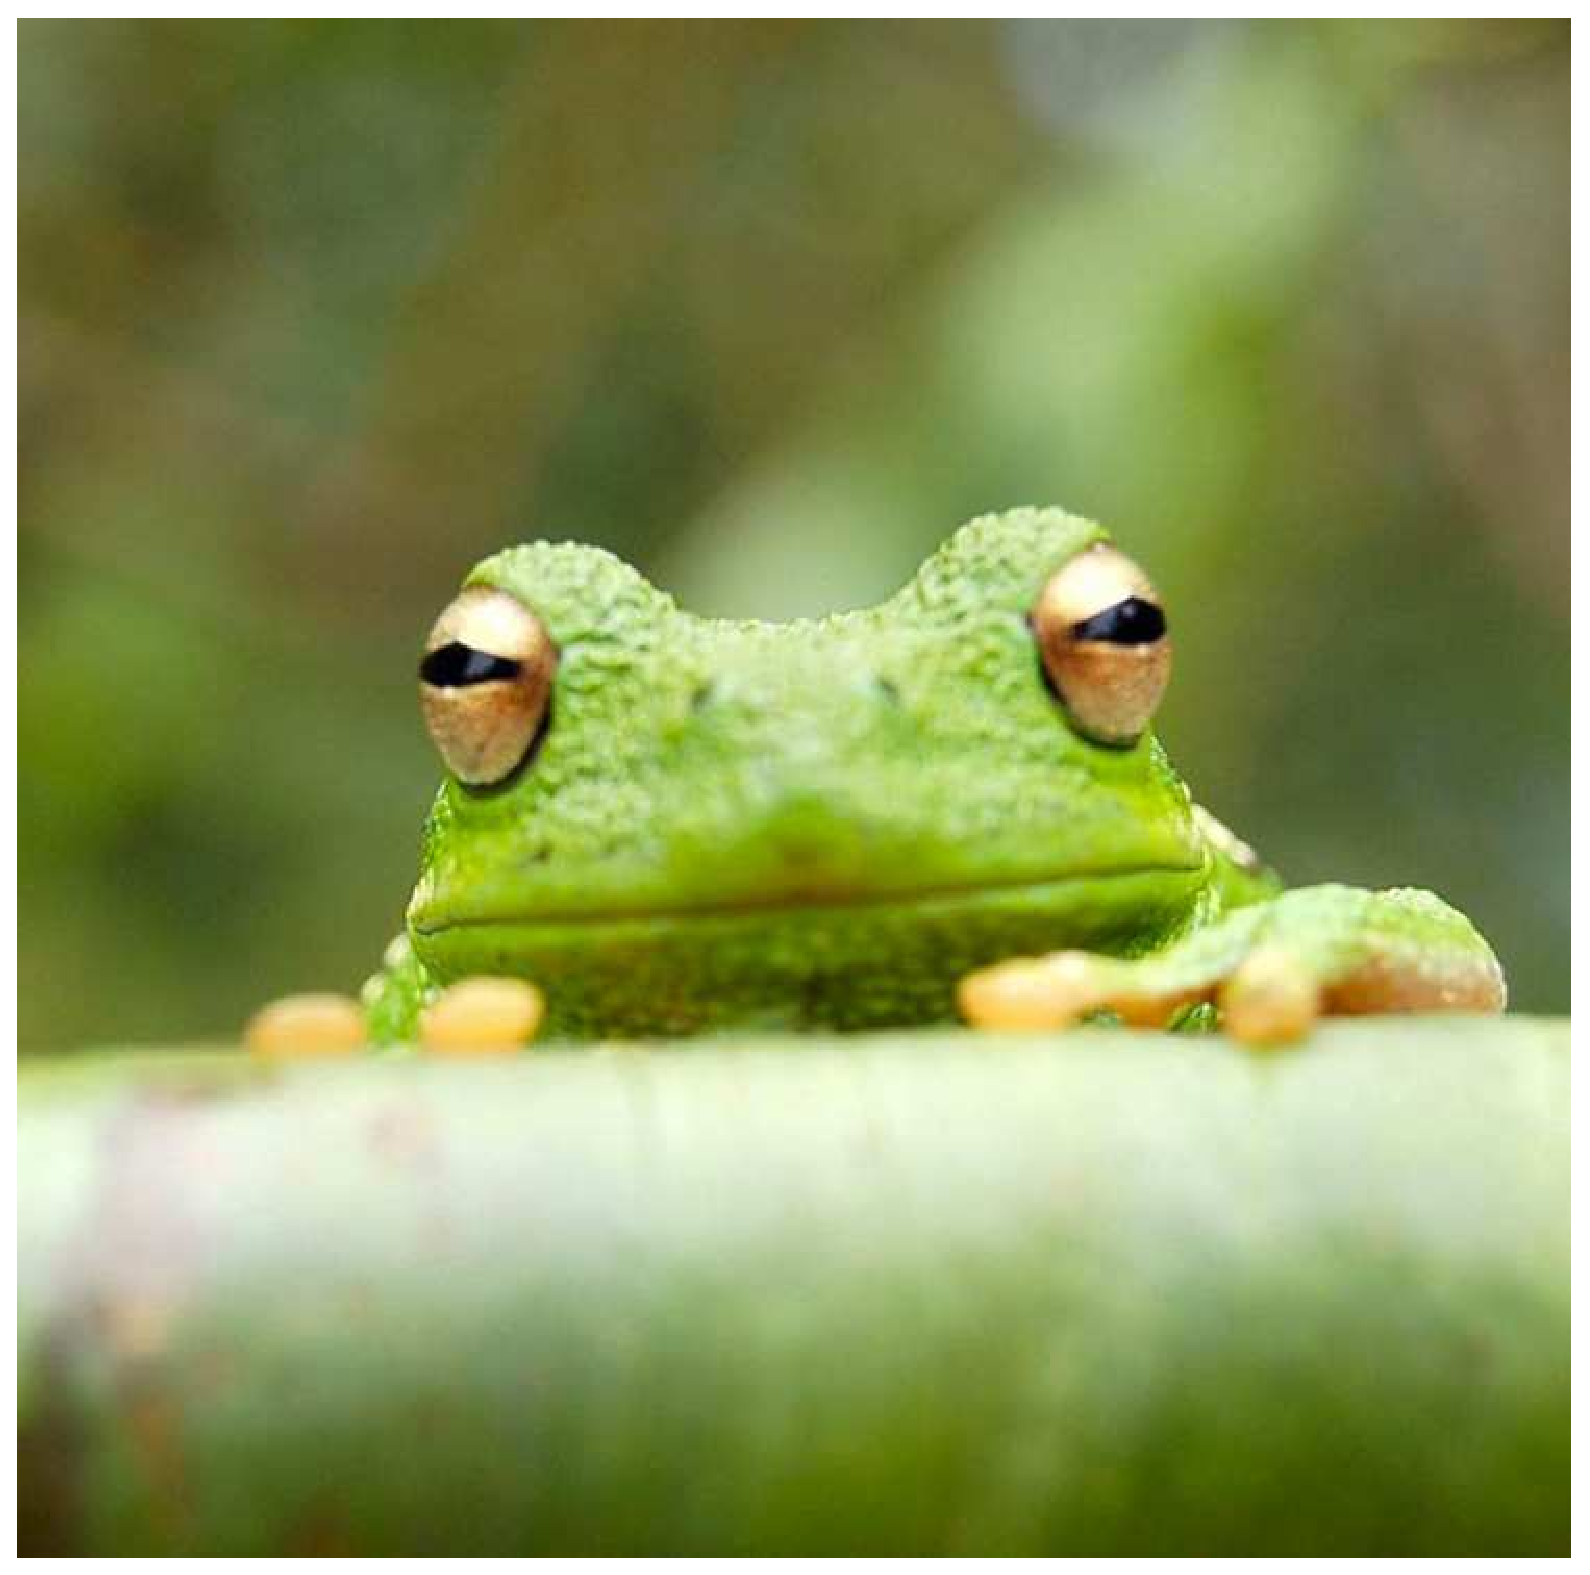
\includegraphics[width=.8\linewidth]{Figures/frog.eps}
\caption{Placeholder image of a frog with a long example legend to show justification setting.}
\label{fig:frog}
\end{figure}


\begin{SCfigure*}[\sidecaptionrelwidth][t]
\centering
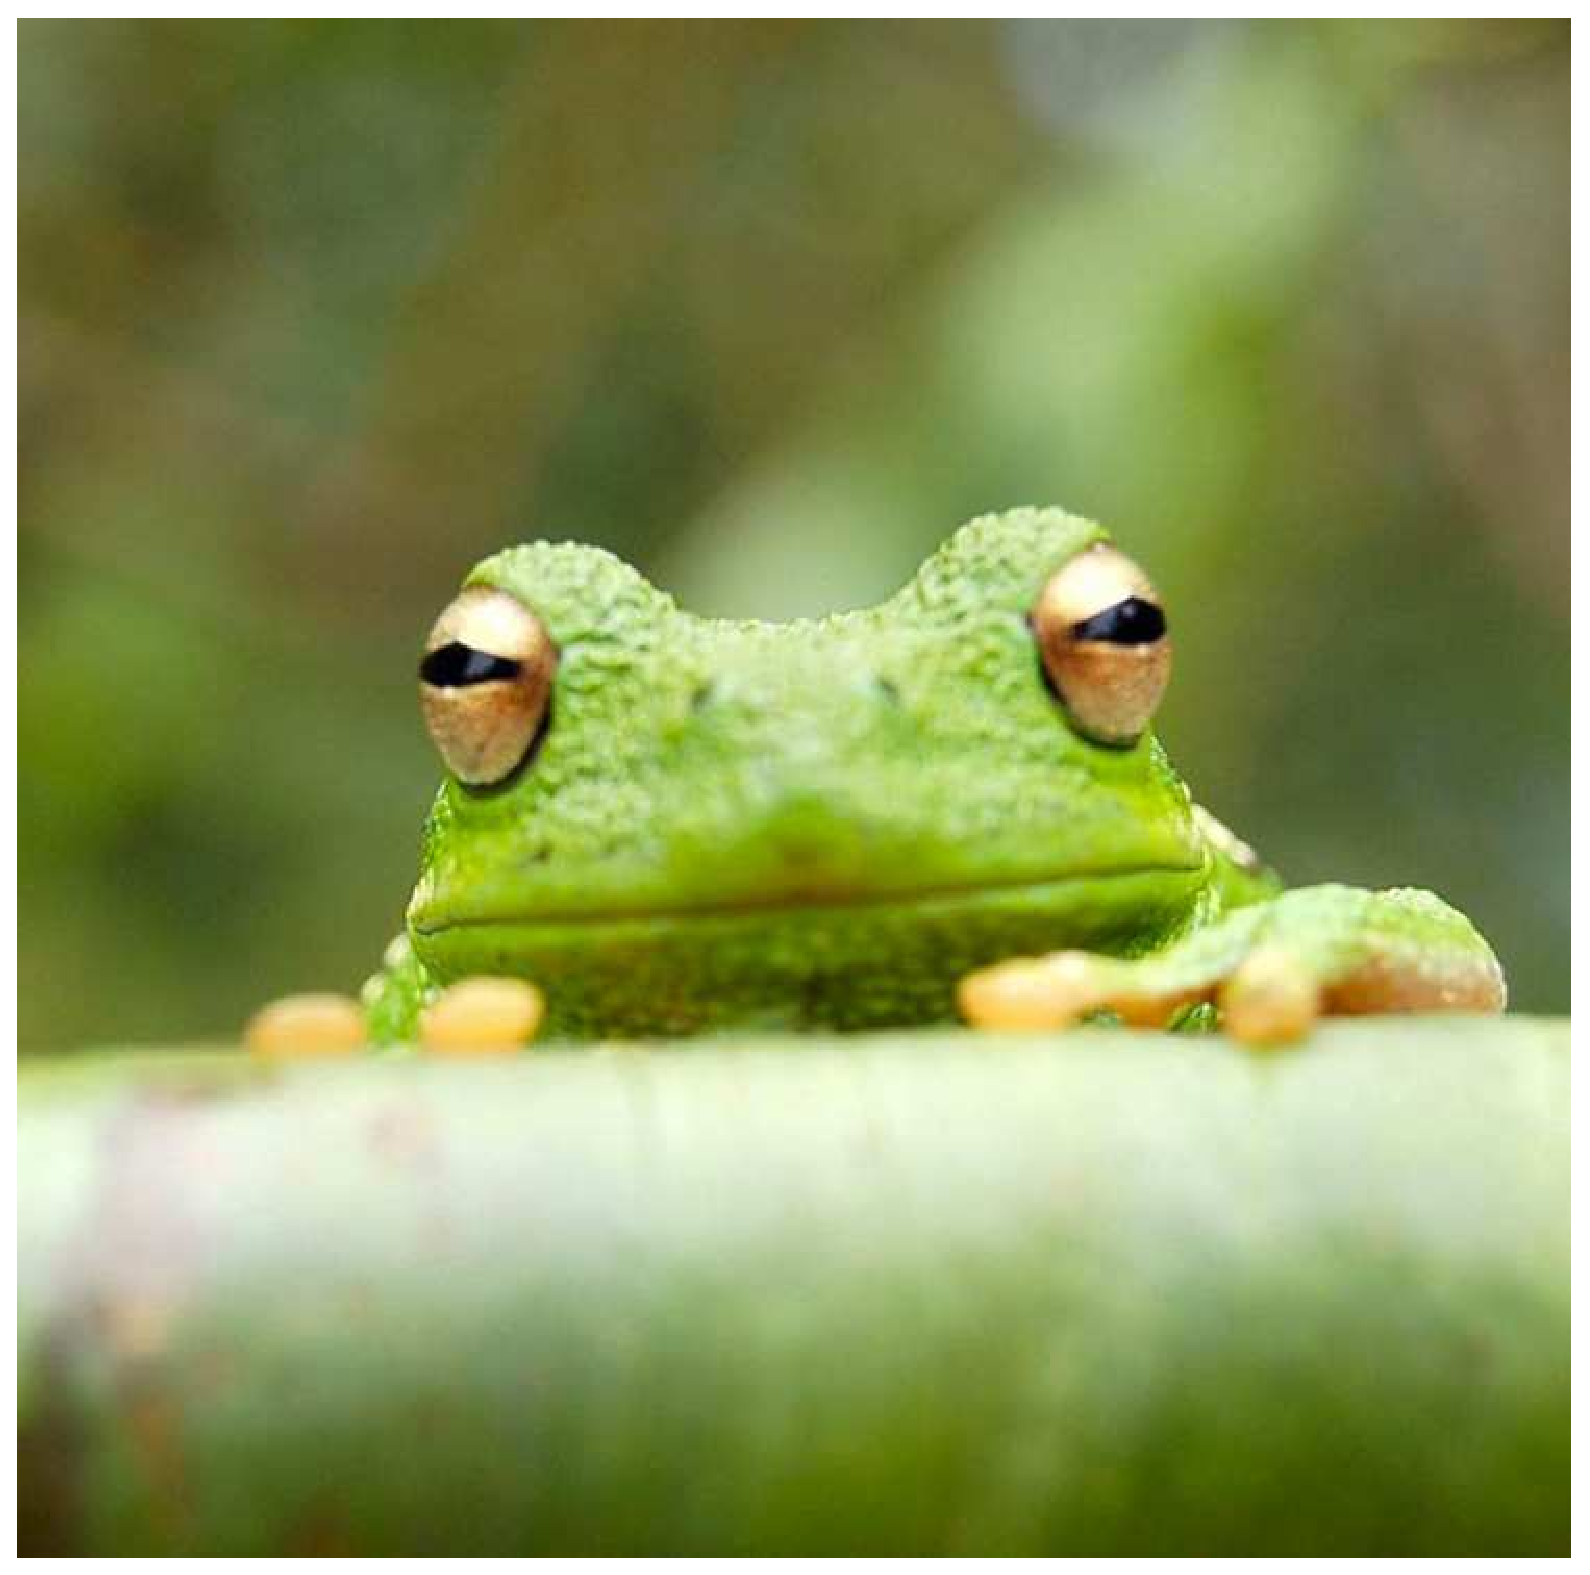
\includegraphics[width=11.4cm,height=11.4cm]{Figures/frog.eps}
\caption{This legend would be placed at the side of the figure, rather than below it.}\label{fig:side}
\end{SCfigure*}

\subsection*{Digital Figures}

Make sure that your figures are of high enough resolution to show up nicely in the document. EPS and high-resolution PDF are usually best, but representations in JPG and PNG can also be used.

 Numbers, letters, and symbols in figures should be large enough to be easily readable within the document. This includes axis labels.

Figures and tables should be labelled and referenced in the standard way using the \verb|\label{}| and \verb|\ref{}| commands.

Figure \ref{fig:frog} shows an example of how to insert a column-wide figure. To insert a figure wider than one column, please use the \verb|\begin{figure*}...\end{figure*}| environment. Figures wider than one column should be sized to 11.4 cm or 17.8 cm wide. Use \verb|\begin{SCfigure*}...\end{SCfigure*}| for a wide figure with side legends.

\subsection*{Tables}
Tables can be included in the main manuscript file, if desired.

\subsection*{Single column equations}

Here is an equation with equation numbering:
\begin{equation}
    (x+y)^3=(x+y)(x+y)^2,
    \label{eqn:myequation}
\end{equation}
and here is a multi-line equation where only one equation is numbered:
\begin{align*}
(x+y)^3&=(x+y)(x+y)^2\\
       &=(x+y)(x^2+2xy+y^2) \numberthis \label{eqn:example} \\
       &=x^3+3x^2y+3xy^3+x^3. 
\end{align*}

Please refer to your equations (e.g., \eqref{eqn:myequation} and \eqref{eqn:example}).

\begin{table}%[tbhp]
\centering
\caption{Comparison of the fitted potential energy surfaces and ab initio benchmark electronic energy calculations}
\begin{tabular}{lrrr}
Species & CBS & CV & G3 \\
\midrule
1. Acetaldehyde & 0.0 & 0.0 & 0.0 \\
2. Vinyl alcohol & 9.1 & 9.6 & 13.5 \\
3. Hydroxyethylidene & 50.8 & 51.2 & 54.0\\
\bottomrule
\end{tabular}

\addtabletext{nomenclature for the TSs refers to the numbered species in the table.}
\end{table}

\subsection*{Supporting Information Appendix (SI)}

Authors may submit SI as a single separate SI Appendix PDF file, with combined text, figures, tables, and SI references. This does not have to follow any special formatting (e.g., you can use the standard LaTeX article class).

Authors who place detailed materials and methods in an SI Appendix must provide sufficient detail in the main text methods to enable a reader to follow the logic of the procedures and results and also must reference the SI methods. 

\subsubsection*{SI Datasets} 

Supply .xlsx, .csv, .txt, .rtf, or .pdf files. 

\acknow{If you wish, you can include any acknowledgments here, set in a single paragraph.}

\showacknow % Display the acknowledgements section

% Bibliography
\bibliography{References}

\end{document}
